% !TEX root = ../main.tex
\chapter{Noise analysis of PSR~J1640+2224} \label{chpt:risultati}

\section{Real data} \label{sec:reali}

\subsection{Validation of Discovery} \label{sec:validazione}

All the analyses of this thesis are performed with \textsc{Discovery}. Since
it is a recent code, we first verify that it reproduces the results of
\textsc{Enterprise}, the reference software introduced in
Section~\ref{sec:software}. We analyze the DR2low data of PSR~J1640+2224
with both codes, using the reference noise model of Section~\ref{NM}, the
priors of Section~\ref{sec:bayes} and the same sampler, so that the only
difference is the implementation of the likelihood.

The posterior distributions are compared in
Figure~\ref{fig:disc_vs_ent}. The contours obtained with the two codes
overlap in all the panels, and so do the one-dimensional posteriors on the
diagonal. The parameter estimates are also in agreement. For example, the
amplitude of the intrinsic red noise is
$\log_{10}A_{\rm RN} = -13.24^{+0.09}_{-0.10}$ with both codes (here and in
the following we quote the median and the $68\%$ credible interval).
The largest difference is found for the spectral index of the DM variations,
$\gamma_{\rm DM} = 4.12^{+2.33}_{-2.28}$ with \textsc{Discovery} and
$\gamma_{\rm DM} = 3.94^{+2.48}_{-2.12}$ with \textsc{Enterprise}, and it is
much smaller than the width of the posterior. The effective number of
samples of Eq.~\eqref{eq:neff} is $1141$ for the \textsc{Discovery} chain and
$1557$ for the \textsc{Enterprise} one, so differences of this size are
expected from the finite length of the chains.

We conclude that \textsc{Discovery} reproduces the results of
\textsc{Enterprise} for this model, and we use it for all the following
analyses.

\begin{figure}[H]
    \centering
    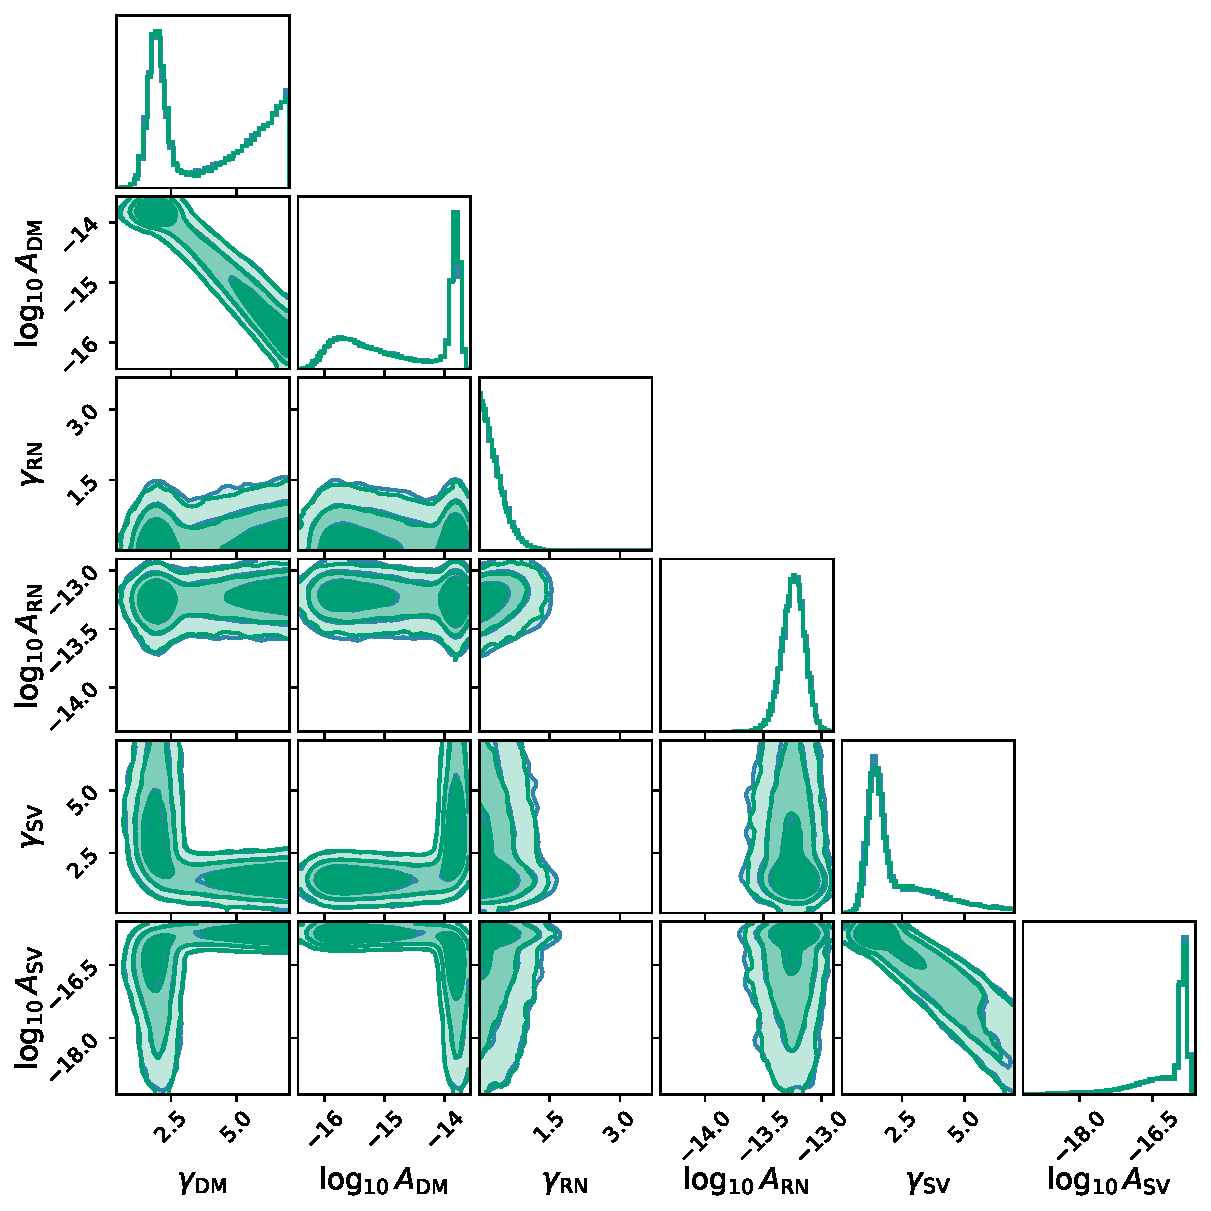
\includegraphics[width=0.75\textwidth]{Figure/cap5/01_discovery_vs_enterprise.pdf}
    \caption{Posterior distributions of the six noise parameters of
    PSR~J1640+2224 obtained from the DR2low data with \textsc{Discovery}
    (blue) and with \textsc{Enterprise} (green). The contours enclose $68\%$,
    $95\%$ and $99.7\%$ of the probability.}
    \label{fig:disc_vs_ent}
\end{figure}

\subsection{DR2low and DR2new+} \label{sec:dr2new}

To show the role of the low radio frequencies, we repeat the analysis on
the DR2new+ dataset, which contains only the observations of the EPTA
telescopes at 1.3--2.6\,GHz, without the LOFAR data. The noise model, the
number of Fourier components and the priors are the same used for DR2low.

The two posterior distributions are compared in
Figure~\ref{fig:dr2low_vs_dr2new}. With DR2new+ none of the parameters of
the chromatic processes is constrained. The posteriors of
$\gamma_{\rm DM}$ and $\gamma_{\rm SV}$ cover the whole prior range, and
those of the amplitudes extend from the lower bound of the prior up to
$\log_{10}A \simeq -13$, so that the data only exclude the largest
amplitudes. The same happens for the intrinsic red noise. In the band of
DR2new+ the chromatic factor of Eq.~\eqref{eq:chrom} is of order one for
both chromatic processes, so they are hard to distinguish from the
achromatic red noise and from each other.

With DR2low the posteriors are much narrower. The LOFAR observations are
at radio frequencies about ten times lower, where the DM variations and
the scattering variations are much stronger and depend on $\nu$ in
different ways, and this allows the chromatic processes to be separated
from the achromatic red noise. The amplitude of the intrinsic red noise,
for example, is unconstrained with DR2new+, while with DR2low it is
$\log_{10}A_{\rm RN} = -13.24^{+0.09}_{-0.10}$. A good coverage in radio
frequency is therefore necessary to measure the chromatic noise of this
pulsar.

\begin{figure}[H]
    \centering
    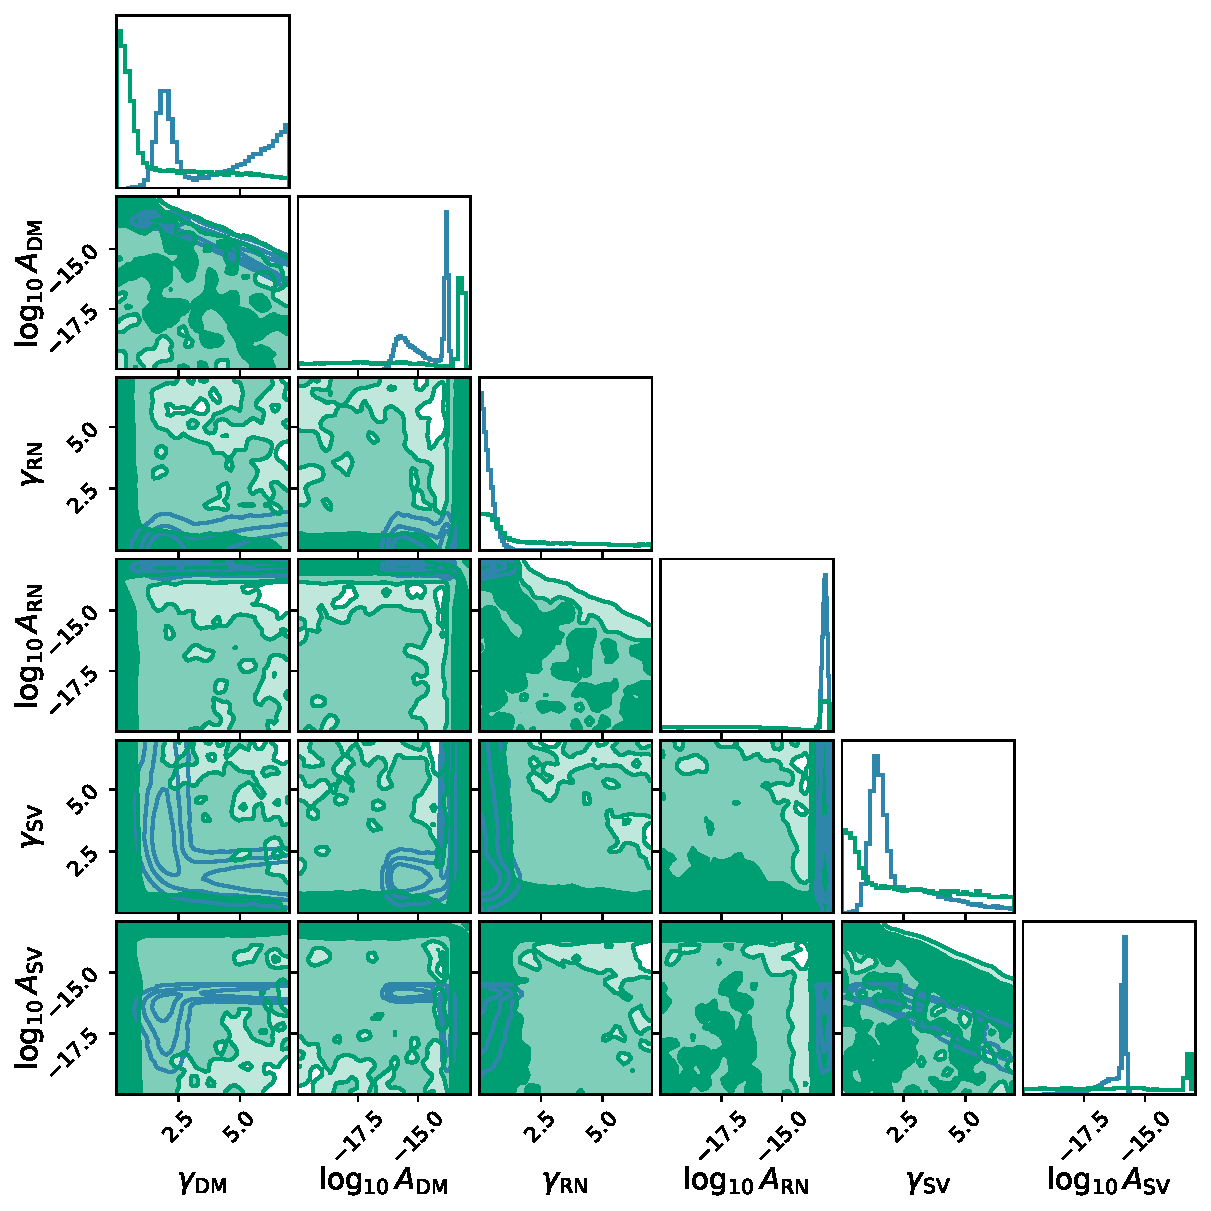
\includegraphics[width=0.75\textwidth]{Figure/cap5/02_DR2low_vs_DR2newplus.pdf}
    \caption{Posterior distributions of the six noise parameters of
    PSR~J1640+2224 obtained from the DR2low data (blue) and from the DR2new+
    data (green). The contours enclose $68\%$, $95\%$ and $99.7\%$ of the
    probability.}
    \label{fig:dr2low_vs_dr2new}
\end{figure}

\subsection{The DM--scattering degeneracy} \label{sec:degenerazione}

We now look in more detail at the DR2low posterior of
Figure~\ref{fig:disc_vs_ent}. The intrinsic red noise is well constrained
and its posterior has a single peak. The DM variations behave differently.
The posteriors of $\gamma_{\rm DM}$ and $\log_{10}A_{\rm DM}$ have two
peaks, one at high amplitude and low spectral index,
$\log_{10}A_{\rm DM} \simeq -13.8$ and $\gamma_{\rm DM} \simeq 2$, and one
at low amplitude, $\log_{10}A_{\rm DM} \simeq -15.5$, where
$\gamma_{\rm DM}$ grows up to the upper bound of the prior. The two peaks
have a comparable weight, so the data do not clearly prefer one of them.
For this reason the median of $\gamma_{\rm DM}$ quoted in
Section~\ref{sec:validazione} falls between the two peaks.

The two peaks are related to the scattering parameters. In the panels that
combine a DM parameter with a scattering parameter the contours are not
ellipses but have the shape of an L. Along one arm the DM variations have
a high amplitude and the scattering is poorly constrained, with a tail
that extends to very low amplitudes. Along the other arm the scattering is
well constrained, $\log_{10}A_{\rm SV} \simeq -15.9$ and
$\gamma_{\rm SV} \simeq 1.4$, and the DM variations are weak. An L-shaped
posterior is the typical sign of a degeneracy between two processes. Here
the chromatic noise at low radio frequencies can be described either
mostly by the DM variations or mostly by the scattering variations, and
the data cannot choose between the two descriptions.

A posterior of the DM parameters with two peaks was also found for this
pulsar in the noise analysis of the DR2low dataset. The origin of this
structure is not known. A possible explanation is that the data contain a
noise process that is not included in the model, and that part of its
power is attributed to the DM variations. In Section~\ref{sec:sim} we
test this hypothesis with simulations.

\subsection{Band noise in the model} \label{sec:bn_reali}

We then add to the noise model the band noise of Section~\ref{sec:bn},
which acts only on the TOAs of the LOFAR band. The model has now eight free
parameters, the six of the reference model plus the amplitude
$A_{\rm BN}$ and the spectral index $\gamma_{\rm BN}$ of the band noise. In
this analysis the scattering variations are modeled with $\alpha = 4.4$,
and the comparison is made with the six-parameter analysis that uses the
same chromatic index.

The posterior distribution is shown in Figure~\ref{fig:reali_8par}. The
parameters of the band noise are not constrained. The posterior of
$\gamma_{\rm BN}$ covers the whole prior range, and that of
$\log_{10}A_{\rm BN}$ extends down to the lower bound of the prior and
drops only at the highest amplitudes. The data therefore give only an
upper limit on the amplitude of the band noise, which at $95\%$
probability is $\log_{10}A_{\rm BN} < -12.21$.

The posteriors of the other six parameters are the same as those obtained
without the band noise in the model. In particular, the two peaks of the DM
parameters and the L-shaped contours between the DM and the scattering
parameters are still present. Adding the band noise to the model therefore
does not remove the degeneracy described in
Section~\ref{sec:degenerazione}.

Since only an upper limit is obtained, the presence of band noise in the
data cannot be excluded. In Section~\ref{sec:sim} we use simulations to
study the effect of a band noise that is present in the data but is not
detected.

\begin{figure}[H]
    \centering
    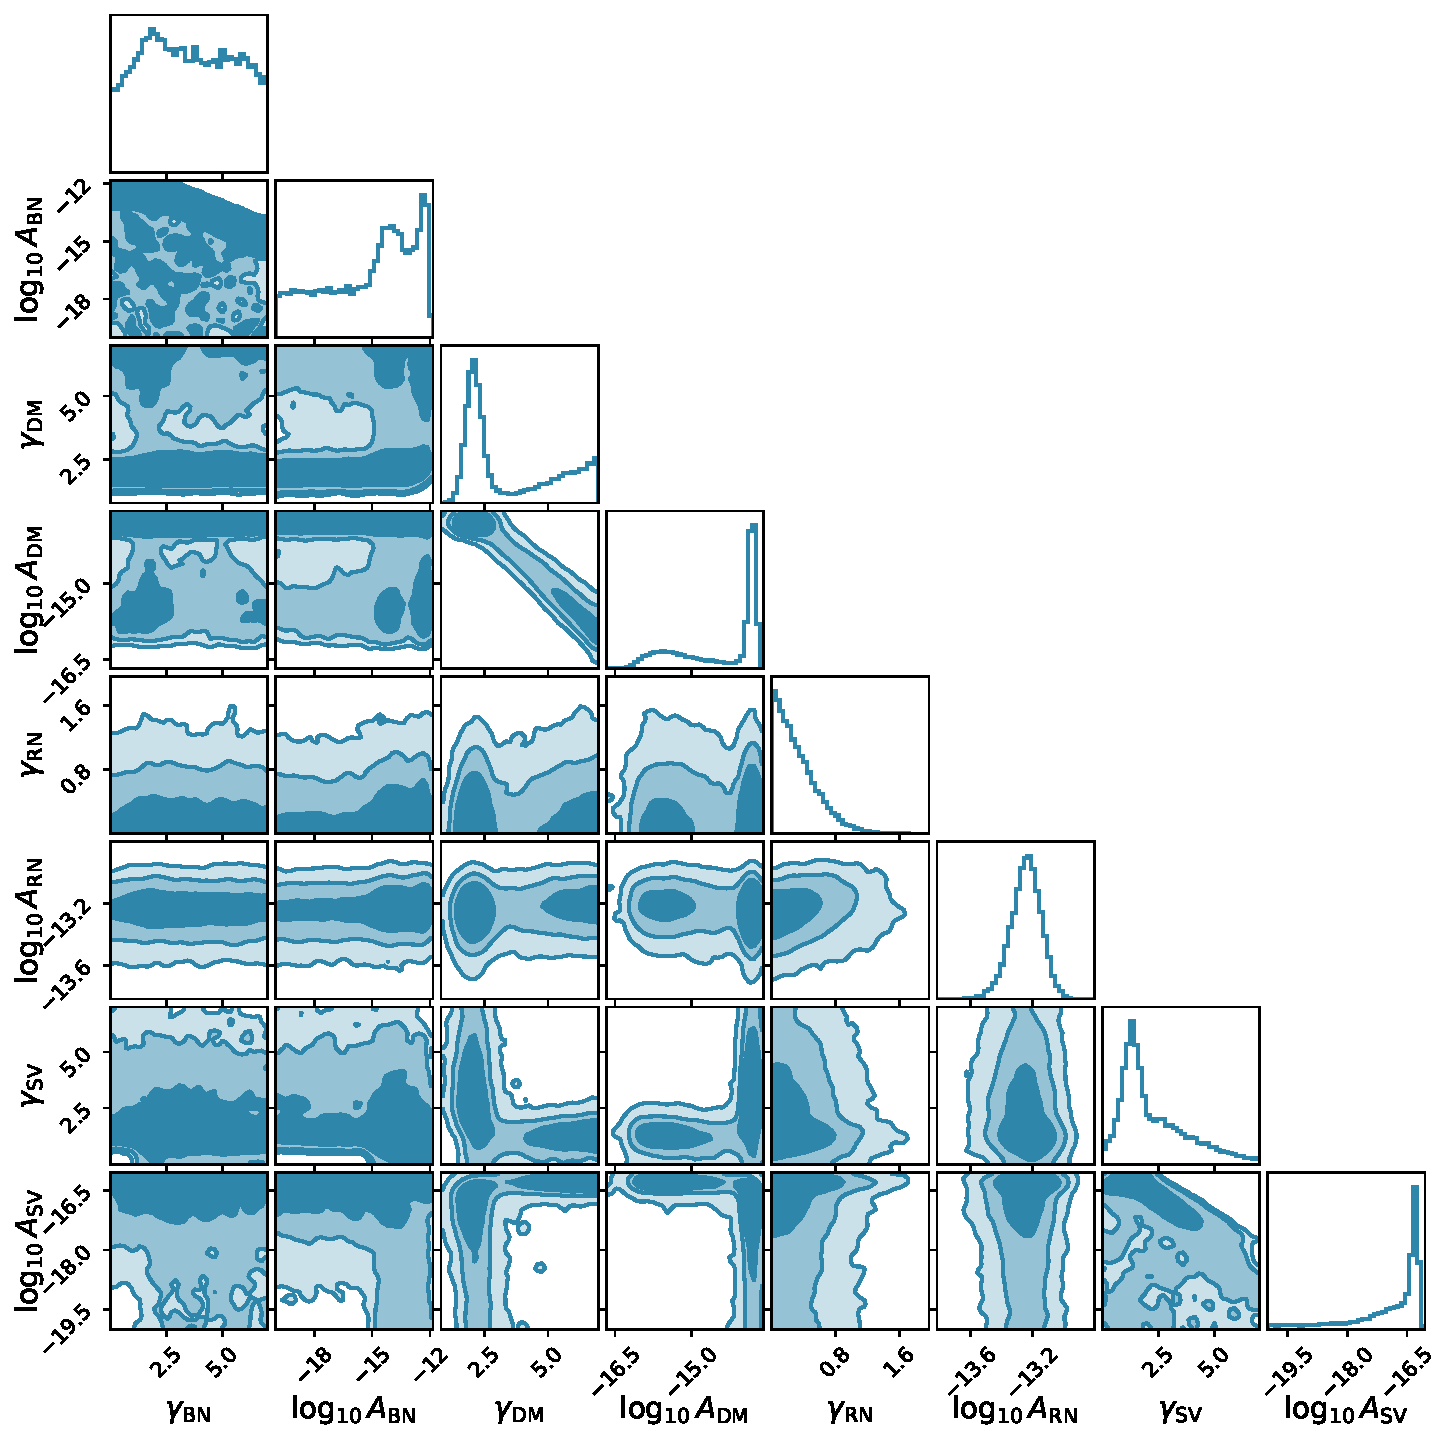
\includegraphics[width=0.75\textwidth]{Figure/cap5/03_reali_8par_band.pdf}
    \caption{Posterior distributions of the eight parameters of the noise
    model with band noise, obtained from the DR2low data of PSR~J1640+2224.
    The contours enclose $68\%$, $95\%$ and $99.7\%$ of the probability.}
    \label{fig:reali_8par}
\end{figure}

\section{Simulations} \label{sec:sim}

To understand the origin of the degeneracy observed in the real data, we
analyze simulated datasets in which the noise content is known. Each
simulated dataset has the same TOAs, TOA uncertainties and observing radio
frequencies as the DR2low data of PSR~J1640+2224, and the same white noise
parameters. The timing residuals are replaced by a random realization of
the noise model, in which each red noise process is a Gaussian process
with the power-law PSD of Chapter~\ref{chpt:rumore} and with chosen values
of its amplitude and spectral index, which we call the injected values.
The simulated data are then analyzed exactly as the real data. Since the
injected values are known, we can check whether they are recovered, and
how the posterior changes when the data contain a process that is not
included in the model.

\subsection{Reference simulation} \label{sec:sim_ref}

In the first simulation the data contain only the three processes of the
reference model, the intrinsic red noise, the DM variations and the
scattering variations with $\alpha = 4$, and they are analyzed with the
same six-parameter model. The model used in the analysis is therefore the
correct one. The posterior is compared with that of the real data in
Figure~\ref{fig:reali_vs_sim}.

All the injected values are recovered, since they lie inside the $95\%$
contours in every panel. The posterior of the simulated data is different
from that of the real data. The DM parameters have a single peak, and the
contours between the DM and the scattering parameters are not L-shaped.
The scattering parameters are well constrained, without the tail toward
low amplitudes seen in the real data. When the data contain only the
processes included in the model, the degeneracy of
Section~\ref{sec:degenerazione} therefore does not appear. In the
following sections we add to the simulated data a process that is not
included in the model, and we study its effect on the posterior.

\begin{figure}[H]
    \centering
    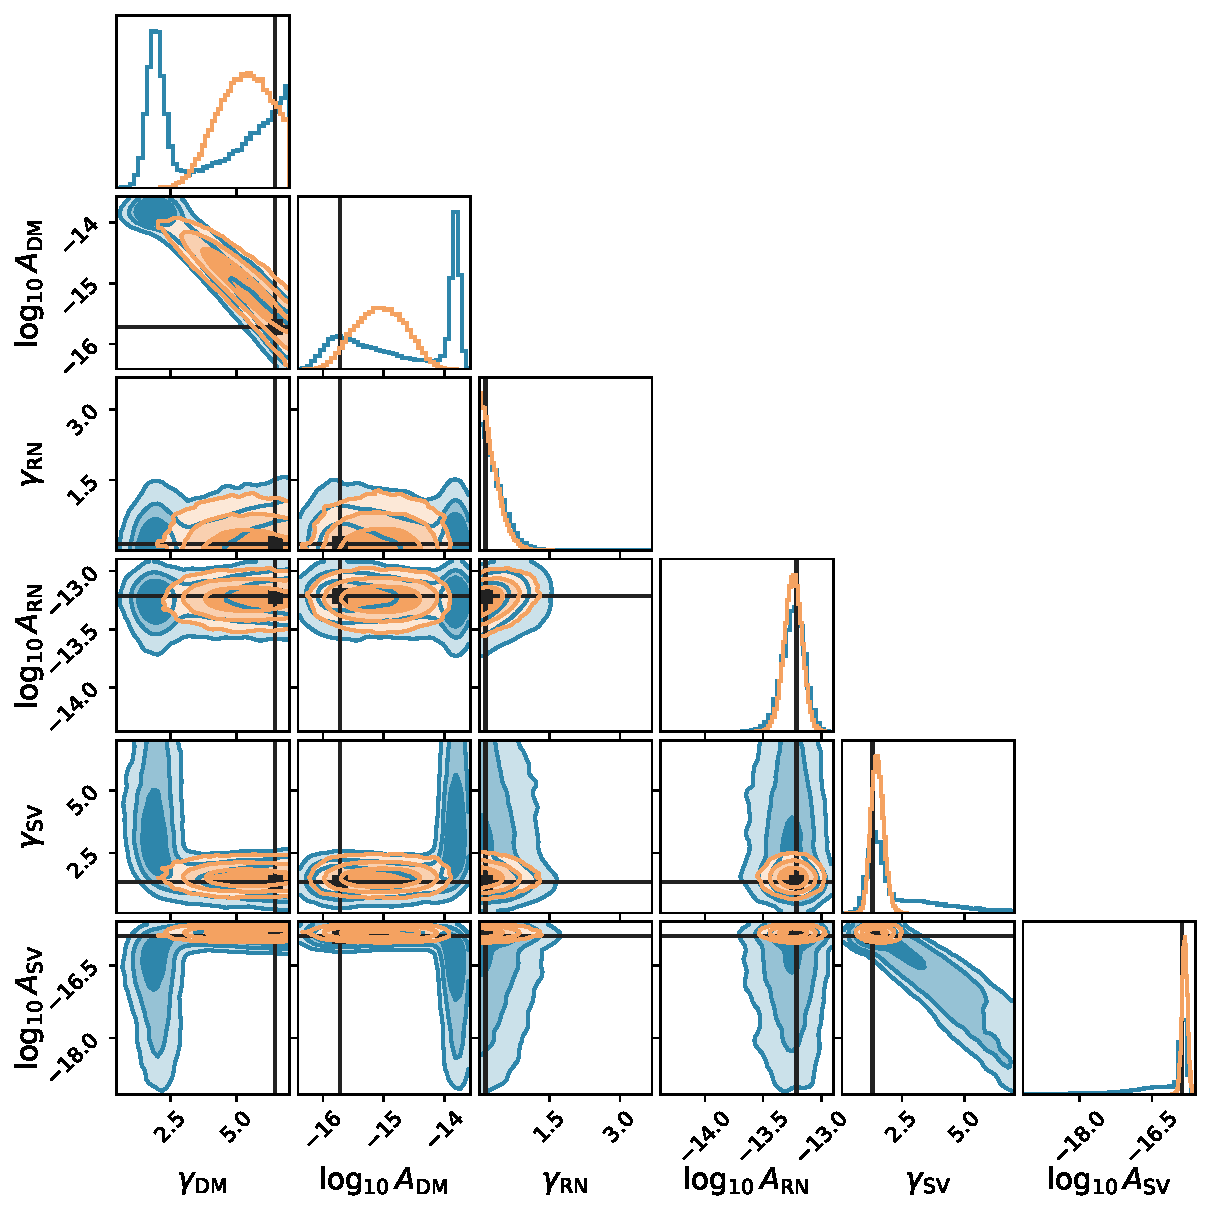
\includegraphics[width=0.75\textwidth]{Figure/cap5/05_reali_vs_simulati.pdf}
    \caption{Posterior distributions of the six noise parameters obtained
    from the DR2low data of PSR~J1640+2224 (blue) and from the reference
    simulation (orange). The black lines mark the injected values. The
    contours enclose $68\%$, $95\%$ and $99.7\%$ of the probability.}
    \label{fig:reali_vs_sim}
\end{figure}

\subsection{Unmodeled GWB} \label{sec:sim_gwb}

As discussed in Section~\ref{sec:rn}, in a single pulsar a GWB acts as an
additional achromatic red noise. If it is present in the data but not in
the model, its power must be attributed to the other processes. To study
this effect we add to the reference simulation a GWB with the spectral
index $\gammagwb = 13/3$ of Eq.~\eqref{eq:PSD_GWB} and three different
amplitudes, $\log_{10}\Agwb = -15.5$, $-15$ and $-14.5$, which cover the
range of the amplitudes expected for the background. The simulated data
are analyzed with the six-parameter model, which does not contain a GWB.

Figure~\ref{fig:sim_gwb} compares the posterior of the simulation with
$\log_{10}\Agwb = -14.5$ with that of the reference simulation. The
injected values of the three noise processes are still recovered. The
intrinsic red noise becomes slightly stronger and steeper, as expected if
it absorbs part of the power of the GWB, but the change is small compared
with the width of the posterior.

\begin{figure}[H]
    \centering
    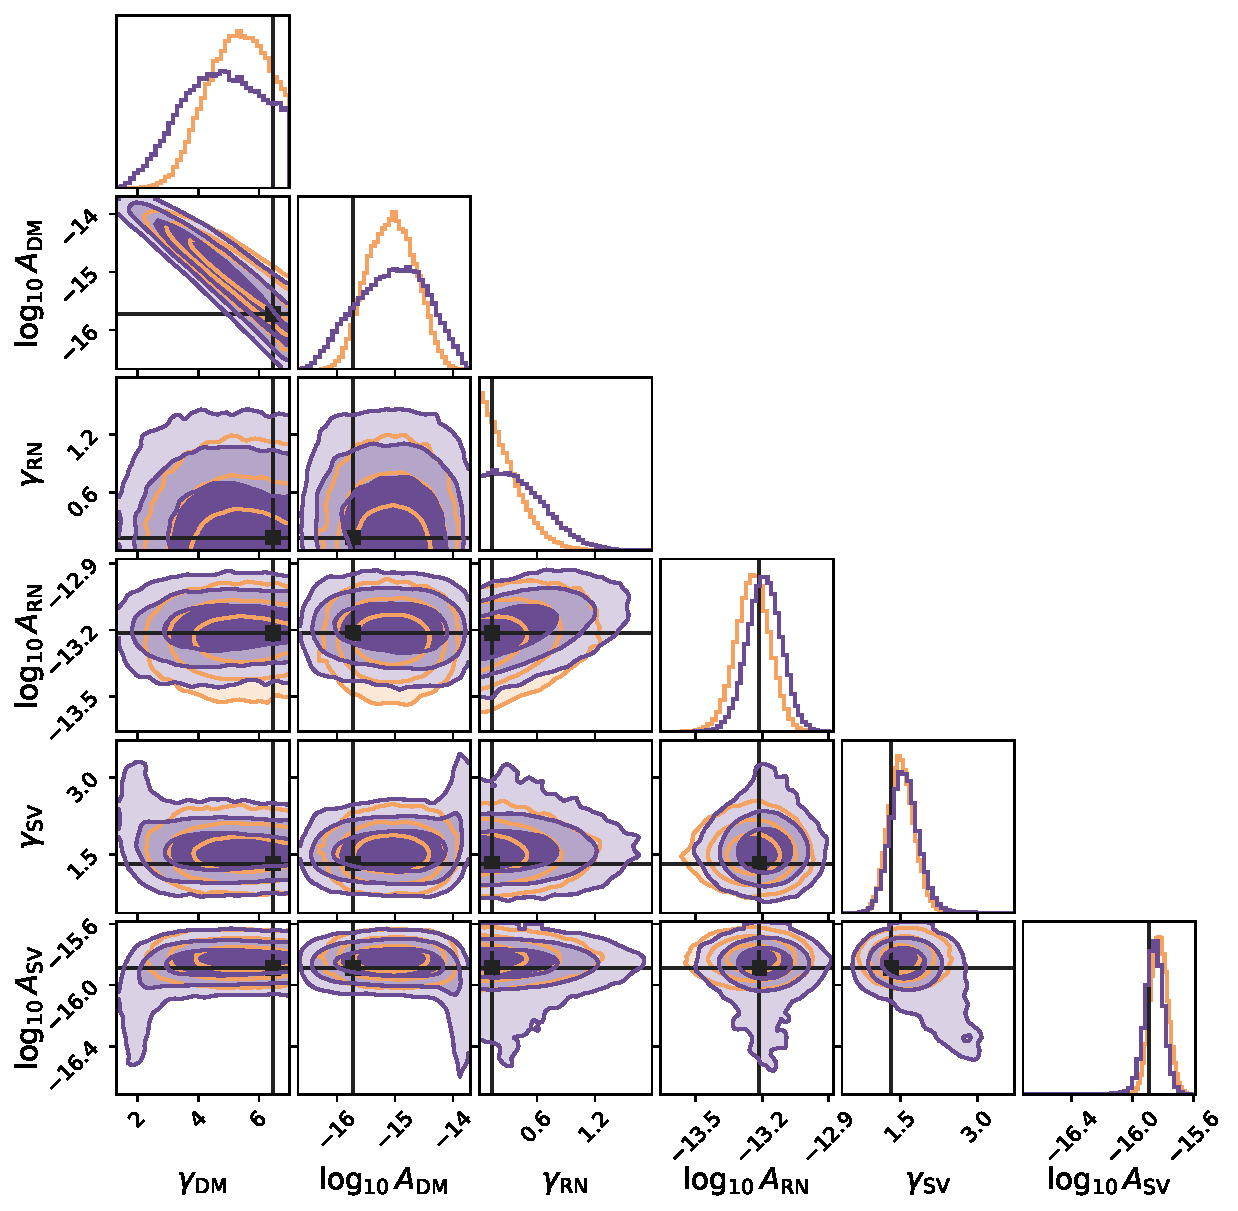
\includegraphics[width=0.75\textwidth]{Figure/cap5/06_sim_noGWB_vs_gwb_A145.pdf}
    \caption{Posterior distributions obtained from the reference simulation
    (orange) and from the simulation with a GWB of amplitude
    $\log_{10}\Agwb = -14.5$ (purple). The black lines mark the injected
    values. Contours as in Figure~\ref{fig:disc_vs_ent}.}
    \label{fig:sim_gwb}
\end{figure}

The main difference is in the panels that combine the DM and the
scattering parameters. With the GWB in the data, the outermost contours
develop two tails that form an L, similar to the one observed in the real
data and absent in the reference simulation. The effect is however much
weaker than in the real data, where the L-shaped structure contains a
large fraction of the posterior, while here it appears only in the
$99.7\%$ contours. The same tails are found for the three amplitudes, and
in this range they do not grow with the amplitude of the GWB.

\subsection{Unmodeled band noise} \label{sec:sim_bn}

We now consider a band noise in the LOFAR band, modeled as described in
Section~\ref{sec:bn}. We simulate datasets that contain the three
processes of the reference model and a band noise with spectral index
$\gamma_{\rm BN} = 3$ and different amplitudes, and a dataset without band
noise that has the same realization of the other processes. In these
simulations the scattering variations have $\alpha = 4.4$, both in the
data and in the model. The simulated data are first analyzed with the
six-parameter model, which does not contain the band noise.

For amplitudes up to $\log_{10}A_{\rm BN} = -14$ the posterior is the same
as without band noise. For larger amplitudes the band noise biases all the
processes, and most of all the DM variations.
Figure~\ref{fig:sim_bn} shows the case $\log_{10}A_{\rm BN} = -12.5$. The
posterior of the DM parameters moves away from the injected values, toward
higher amplitudes and lower spectral indices, from
$\log_{10}A_{\rm DM} = -15.09^{+0.52}_{-0.48}$ and
$\gamma_{\rm DM} = 5.39^{+1.06}_{-1.25}$ without band noise to
$\log_{10}A_{\rm DM} = -14.03^{+0.14}_{-0.18}$ and
$\gamma_{\rm DM} = 2.69^{+0.67}_{-0.55}$. The intrinsic red noise also
becomes steeper, while the scattering parameters change very little.

\begin{figure}[H]
    \centering
    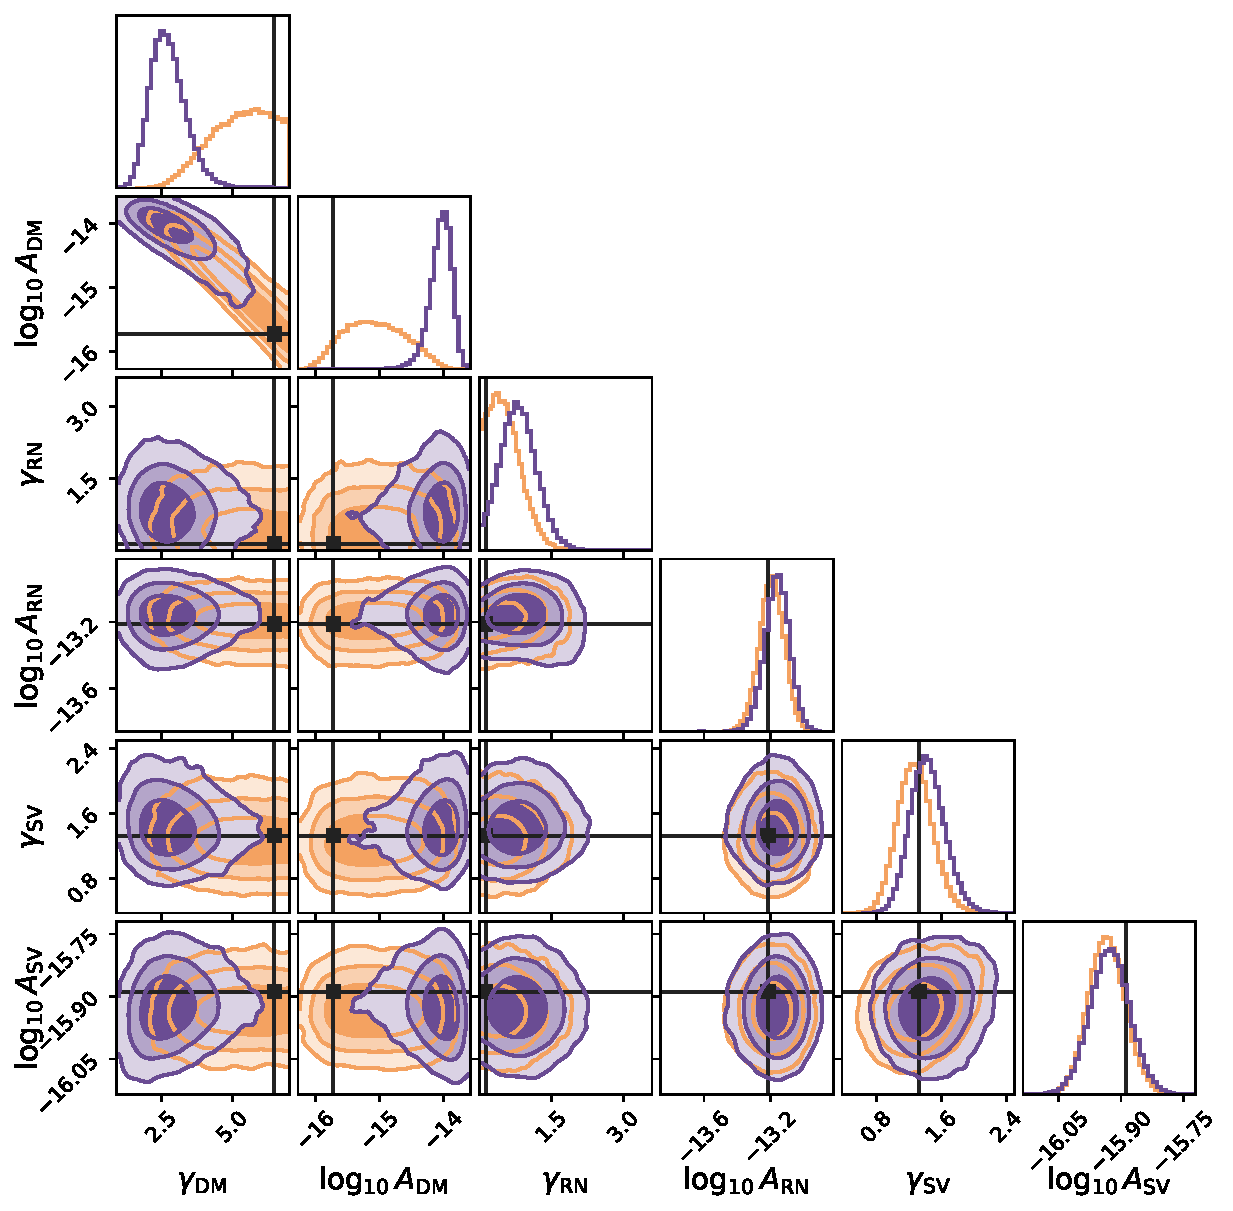
\includegraphics[width=0.75\textwidth]{Figure/cap5/07_bn_A125_6par_OFF_vs_band.pdf}
    \caption{Posterior distributions obtained from the simulation without
    band noise (orange) and from the simulation with a band noise of
    amplitude $\log_{10}A_{\rm BN} = -12.5$ (purple), both analyzed with
    the six-parameter model. The black lines mark the injected values.
    Contours as in Figure~\ref{fig:disc_vs_ent}.}
    \label{fig:sim_bn}
\end{figure}

An unmodeled band noise therefore produces a peak of the DM parameters at
an amplitude and a spectral index close to those of the high-amplitude
peak found in the real data, $\log_{10}A_{\rm DM} \simeq -13.8$ and
$\gamma_{\rm DM} \simeq 2$ (Section~\ref{sec:degenerazione}). In the
simulation, however, the DM posterior has this peak only, and the contours
between the DM and the scattering parameters are not L-shaped. An
unmodeled band noise can thus explain the position of the high-amplitude
peak, but it does not reproduce by itself the whole structure observed in
the real data.

\subsection{Detectability of the band noise} \label{sec:sim_bn_det}

The same simulations are then analyzed with the eight-parameter model of
Section~\ref{sec:bn_reali}, which contains the band noise. For
$\log_{10}A_{\rm BN} = -12.5$ the band noise is not detected. Its
parameters are not constrained, the upper limit on its amplitude is
$\log_{10}A_{\rm BN} < -12.36$ at $95\%$ probability, and the DM
parameters remain biased as in the six-parameter analysis. The band noise
is detected only for $\log_{10}A_{\rm BN} = -12$, where we recover
$\log_{10}A_{\rm BN} = -12.08^{+0.12}_{-0.21}$ and
$\gamma_{\rm BN} = 3.16^{+0.64}_{-0.47}$.

The upper limit obtained from the real data,
$\log_{10}A_{\rm BN} < -12.21$, is similar to the one obtained from the
simulation with $\log_{10}A_{\rm BN} = -12.5$. The real data are therefore
compatible with a band noise of this amplitude, which would not be
detected but would be strong enough to bias the DM parameters. For this
reason the presence of band noise in the real data cannot be excluded.
